\documentclass[tikz,border=15pt]{standalone}
\usetikzlibrary{positioning, shapes.geometric, arrows.meta, fit, backgrounds, calc}

\begin{document}

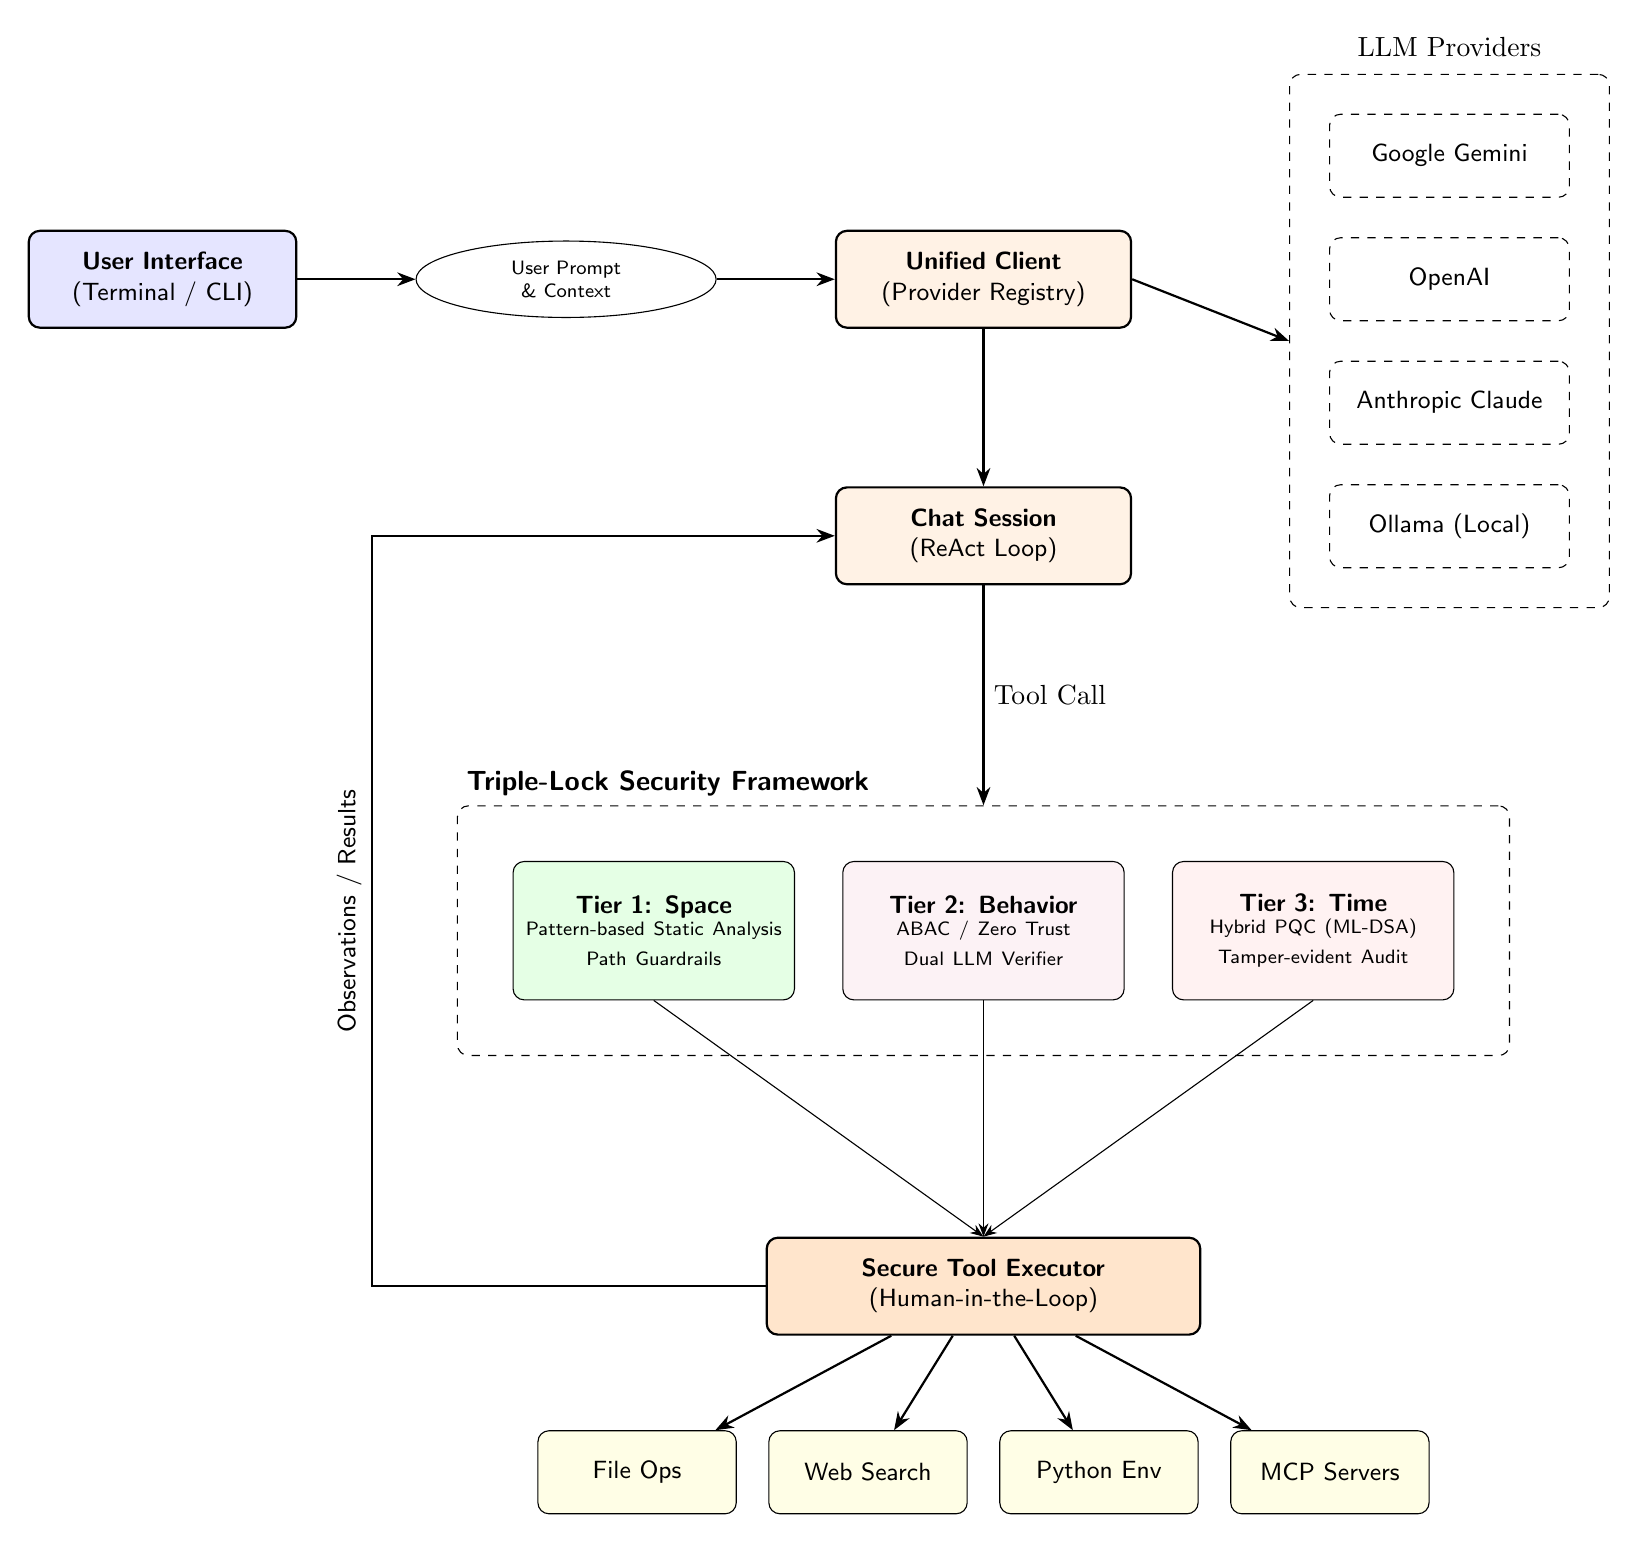
\begin{tikzpicture}[
    node distance=1.5cm and 2cm,
    auto,
    >=Stealth,
    % Styles
    base/.style={rectangle, draw, rounded corners, text centered, minimum height=3.5em, font=\sffamily\small},
    cli/.style={base, fill=blue!10, text width=9em, thick},
    orchestrator/.style={base, fill=orange!10, text width=10em, thick},
    provider/.style={base, fill=white, text width=8em, dashed, minimum height=3em},
    tier/.style={base, text width=9.5em, minimum height=5em},
    tier1/.style={tier, fill=green!10},
    tier2/.style={tier, fill=purple!5},
    tier3/.style={tier, fill=red!5},
    tool/.style={base, fill=yellow!10, text width=6.5em, minimum height=3em},
    data/.style={ellipse, draw, fill=white, text width=7em, text centered, font=\sffamily\scriptsize},
    groupbox/.style={draw, dashed, inner sep=0.5cm, rounded corners, font=\sffamily\bfseries}
]

    % --- Level 1: Interface ---
    \node [cli] (user) {\textbf{User Interface} \\ (Terminal / CLI)};
    \node [data, right=1.5cm of user] (prompt) {User Prompt \\ \& Context};

    % --- Level 2: Core Orchestration ---
    \node [orchestrator, right=1.5cm of prompt] (unified) {\textbf{Unified Client} \\ (Provider Registry)};
    \node [orchestrator, below=2cm of unified] (session) {\textbf{Chat Session} \\ (ReAct Loop)};

    % --- Level 3: LLM Providers ---
    \node [provider, right=2.5cm of unified] (openai) {OpenAI};
    \node [provider, above=0.5cm of openai] (gemini) {Google Gemini};
    \node [provider, below=0.5cm of openai] (claude) {Anthropic Claude};
    \node [provider, below=0.5cm of claude] (ollama) {Ollama (Local)};

    \node [groupbox, fit=(gemini) (ollama), label={[shift={(0,0.1)}]above:LLM Providers}] (llm_group) {};

    % --- Level 4: Security Pipeline (Triple-Lock) ---
    % Positioning Tier 2 first in the center
    \node [tier2, below=3.5cm of session] (t2) {
        \textbf{Tier 2: Behavior} \\ 
        \scriptsize ABAC / Zero Trust \\ 
        \scriptsize Dual LLM Verifier
    };
    \node [tier1, left=0.6cm of t2] (t1) {
        \textbf{Tier 1: Space} \\ 
        \scriptsize Pattern-based Static Analysis \\ 
        \scriptsize Path Guardrails
    };
    \node [tier3, right=0.6cm of t2] (t3) {
        \textbf{Tier 3: Time} \\ 
        \scriptsize Hybrid PQC (ML-DSA) \\ 
        \scriptsize Tamper-evident Audit
    };

    \node [groupbox, fit=(t1) (t3), inner sep=0.7cm] (security_group) {};
    \node [anchor=south west, font=\sffamily\bfseries] at (security_group.north west) {Triple-Lock Security Framework};

    % --- Level 5: Tool Execution ---
    \node [orchestrator, fill=orange!20, below=3cm of t2, text width=15em, thick] (executor) {
        \textbf{Secure Tool Executor} \\ (Human-in-the-Loop)
    };

    % --- Level 6: External Tools ---
    % Center the group of 4 tools by placing the middle two symmetrically
    \node [tool, anchor=north east, xshift=-0.2cm] (web) at ($(executor.south) + (0,-1.2)$) {Web Search};
    \node [tool, anchor=north west, xshift=0.2cm] (python) at ($(executor.south) + (0,-1.2)$) {Python Env};
    \node [tool, left=0.4cm of web] (file) {File Ops};
    \node [tool, right=0.4cm of python] (mcp) {MCP Servers};

    % --- Connections ---
    \draw [->, thick] (user) -- (prompt);
    \draw [->, thick] (prompt) -- (unified);
    \draw [->, thick] (unified) -- (session);
    
    % To LLM
    \draw [->, thick] (unified.east) -- (llm_group.west);
    
    % To Security & Tools
    \draw [->, thick] (session) -- (security_group.north) node [midway, right] {Tool Call};
    
    \draw [->] (t1.south) -- (executor.north);
    \draw [->] (t2.south) -- (executor.north);
    \draw [->] (t3.south) -- (executor.north);
    
    \draw [->, thick] (executor) -- (file);
    \draw [->, thick] (executor) -- (web);
    \draw [->, thick] (executor) -- (python);
    \draw [->, thick] (executor) -- (mcp);

    % Feedback Loop
    \draw [->, thick] (executor.west) -- ++(-5,0) coordinate (P) 
        -- (P |- session.west) node [midway, above, rotate=90, font=\sffamily\small] {Observations / Results} 
        -- (session.west);

\end{tikzpicture}

\end{document}
